\documentclass[11pt]{article}

% ----------------------------------------------------------------------
% LayerScore: Project Design & Preregistration
% Consolidated reference document
% ----------------------------------------------------------------------

\usepackage{lmodern}
\usepackage[T1]{fontenc}
\usepackage[utf8]{inputenc}
\usepackage[a4paper,margin=1in]{geometry}
\usepackage{amsmath,amssymb}
\usepackage{booktabs}
\usepackage{array}
\usepackage{tabularx}
\usepackage{xcolor}
\usepackage{enumitem}
\usepackage{microtype}
\usepackage{caption}
\usepackage{tikz}
\usetikzlibrary{shapes.geometric,arrows.meta,positioning,calc,fit,backgrounds}
\usepackage[colorlinks=true,linkcolor=teal!70!black,urlcolor=blue!60!black,citecolor=teal!70!black]{hyperref}

% --- palette ---
\definecolor{lsblue}{HTML}{2C6E9B}
\definecolor{lsgreen}{HTML}{2E7D5B}
\definecolor{lsred}{HTML}{B4453C}
\definecolor{lsgray}{HTML}{F1F3F5}
\definecolor{lsamber}{HTML}{B07A1E}

% --- class-name shortcuts (consistent typesetting, safe underscores) ---
\newcommand{\Ccar}{\texttt{rna\_to\_protein}}
\newcommand{\Cinv}{\texttt{protein\_inverted}}
\newcommand{\Crna}{\texttt{rna\_only\_supported}}
\newcommand{\Cpho}{\texttt{phospho\_residual}}
\newcommand{\Cind}{\texttt{indeterminate}}
\newcommand{\Cphoalt}{\texttt{phospho\_altered}}
\newcommand{\breakuscore}{\textunderscore\allowbreak}
\newcommand{\code}[1]{\texttt{\small\let\_\breakuscore #1}}
\emergencystretch=2em

\newcolumntype{L}{>{\raggedright\arraybackslash}X}

\captionsetup{font=small,labelfont=bf}
\setlist{nosep,leftmargin=1.4em}

% --- tikz styles ---
\tikzset{
  start/.style={rounded corners, draw=lsblue!80, fill=lsblue!8, line width=0.6pt,
    align=center, inner sep=5pt, font=\small},
  decide/.style={diamond, aspect=2.1, draw=lsamber!85, fill=lsamber!10, line width=0.6pt,
    align=center, inner sep=1pt, font=\scriptsize, text width=2.5cm},
  termgood/.style={rounded corners, draw=lsgreen!75, fill=lsgreen!10, line width=0.7pt,
    align=center, inner sep=4pt, font=\scriptsize\ttfamily, text width=2.5cm},
  termstop/.style={rounded corners, draw=lsred!75, fill=lsred!10, line width=0.7pt,
    align=center, inner sep=4pt, font=\scriptsize\ttfamily, text width=2.5cm},
  gate/.style={rounded corners, draw=lsblue!80, fill=lsblue!7, line width=0.7pt,
    align=left, inner sep=6pt, font=\small, text width=10.6cm},
  stopnode/.style={rounded corners, draw=lsred!75, fill=lsred!10, line width=0.7pt,
    align=center, inner sep=4pt, font=\scriptsize, text width=2.3cm},
  flow/.style={-{Stealth[length=2.4mm]}, line width=0.6pt},
  lbl/.style={font=\scriptsize\itshape, fill=white, inner sep=1pt},
}

\title{\vspace{-1.2cm}\textbf{LayerScore}\\[2pt]
\large A Calibrated Estimand for Cross-Layer Signal Localization\\ in Matched Multi-Omics\\[6pt]
\normalsize\textit{Project Design, Methodology, and Preregistration}}
\author{Ibrahim Shahid}
\date{19 July 2026 \quad\textbar\quad Version 0.1 (design-freeze candidate)}

\begin{document}
\maketitle
\vspace{-0.6cm}

\begin{abstract}
\noindent This document consolidates the full design of \textbf{LayerScore}, a statistical method that,
for a controlled biological contrast with matched RNA, protein, and (optionally) phosphoproteomic
measurements, decides \emph{which molecular layer carries the response of each pathway}. Unlike existing
multi-omic integrators, which fuse layers or rank their contribution to a combined score, LayerScore
returns a per-pathway \emph{decision} drawn from a small label set --- concordant carriage, protein
inversion, supported RNA-only response, residual phosphoregulation, or explicit abstention --- each backed
by an observability-matched null and, critically, distinguishing \emph{supported absence of protein
carriage} from \emph{insufficient evidence}. The document states the estimands and their known statistical
hazards, the classification rules, the novelty boundary against MOGSA / ActivePathways / MOFA+, the
validation hierarchy (simulation first, spaceflight last), the datasets, and a gated execution plan with
preregistered null interpretations. It is a companion to the kidney biology manuscript (``v12''); the two
share code and data but make disjoint claims.
\end{abstract}

\tableofcontents
\vspace{0.4cm}

% ======================================================================
\section{Purpose of this document}
This is a single reference artifact for the LayerScore project. It merges the strategic rationale, the
formal method, the corrections identified in review, the validation plan, and the data manifest into one
citable specification. It is written to double as a \emph{preregistration}: every analysis has a
predeclared endpoint and a null interpretation that is reportable whether or not the result is positive.
Nothing here depends on wet-lab access; the entire program is computational and uses public data.

% ======================================================================
\section{Strategic rationale}

\subsection{The ceiling on the kidney biology story}
The companion kidney study establishes a spaceflight distal-nephron dephosphorylation phenotype and a
recurrent RNA/protein mismatch, but it is bounded by three limits that no additional public-data analysis
can remove: whole-kidney phosphoproteomics cannot localize sites to DCT2/CNT cells; there is no matched
electrolyte or blood-pressure physiology, so transport function cannot be tied to the molecular pattern;
and simultaneous measurements cannot establish causal ordering. The broadened DCT2/CNT interpretation is
additionally \emph{scoring-sensitive}: under a pure-specificity subtype score the enrichment is modest
(odds ratio ${\approx}1.3$) and only borderline under an observability-matched permutation
($p=0.062$), with a cytoskeletal, non-canonical leading edge. These are biology limits.

\subsection{Why a methods framing changes the burden of proof}
Every limit above constrains a \emph{biological} claim. A methods contribution is validated primarily on
\emph{synthetic data with known truth}, where cell resolution, physiology, and causal ordering are not
required. Reframing the project around the statistical distinction --- rather than around the RNA/protein
mismatch as a discovery --- moves the load-bearing evidence onto ground the author can fully control, and
demotes the fragile kidney result from ``flagship discovery'' to ``illustrative capability demonstration.''
This is the central reason to pivot: not that LayerScore is more novel than the biology, but that it is
\emph{defensible under adversarial questioning} in a way a public-data biology reanalysis is not.

\subsection{Two papers, one codebase}
The project splits cleanly into two deliverables with disjoint claims and a shared implementation. The
methods paper must not re-assert the biology as a second discovery.

\begin{center}\small
\begin{tabularx}{\textwidth}{@{}L L@{}}
\toprule
\textbf{v12 owns (biology)} & \textbf{LayerScore owns (method)} \\
\midrule
Spaceflight kidney biology & A general statistical estimand \\
DCT1 / DCT2 / CNT subtype prioritization & Layer-carriage classification with abstention \\
NCC / WNK / SPAK phosphosite findings & Simulation + benchmark validation of the estimand \\
Kidney-specific mechanistic interpretation & Same-animal cross-tissue specificity test (RR-1) \\
Full OSD-462 biological analysis & Brief OSD-462 demonstration, citing v12 for the biology \\
\bottomrule
\end{tabularx}
\end{center}

\noindent The split is also a hedge: if a referee judges the method's novelty thin, v12 stands on its own;
if the DCT2 biology stays borderline, LayerScore stands on its simulation backbone.

% ======================================================================
\section{The method: what LayerScore estimates}

\subsection{The exact question (the niche)}
For a controlled contrast (here, spaceflight vs.\ ground control), and for each pathway $P$, LayerScore
jointly estimates four things existing tools do not jointly return:
\begin{enumerate}
\item \textbf{Directional carriage}: does the protein response follow the RNA direction?
\item \textbf{Directional inversion}: is the protein response significantly \emph{opposite} to RNA?
\item \textbf{Residual phosphoregulation}: do phosphosites move after accounting for their parent protein?
\item \textbf{Supported absence vs.\ uncertainty}: is protein carriage genuinely near zero, or merely
underpowered / unobservable?
\end{enumerate}
The fourth point is the identity of the method. ``Protein was non-significant'' must not collapse to
\Crna{}. LayerScore separates \emph{supported} RNA-only responses (protein equivalence to zero with
adequate observability) from \Cind{} (insufficient coverage or intervals too wide). This is the distinction
MOGSA cannot make (\S\ref{sec:novelty}).

\subsection{Gene-level inputs and notation}
Each layer contributes a per-feature effect estimate for the flight contrast, with a standard error:
\[
\begin{aligned}
&r_g = \text{RNA flight effect},\ \mathrm{SE}(r_g); \qquad
p_g = \text{protein flight effect},\ \mathrm{SE}(p_g);\\[2pt]
&\beta_{s} = \text{phosphosite $s$ effect}.
\end{aligned}
\]
Let $P$ be a pathway gene set; let $\mathcal{C}_P$ be its \emph{co-observed} genes (RNA and protein both
quantified); let $\mathcal{R}_P=\{g:\text{RNA CI excludes }0\}$ be its \emph{RNA-responsive} subset. Weights
$w_g$ default to inverse variance $w_g = 1/\mathrm{SE}(p_g)^2$; whatever the choice, the matched null
(\S\ref{sec:null}) must be matched on the same quantity that induces $w_g$.

\subsection{Two complementary RNA$\rightarrow$protein estimands}
\textbf{(i) Sign-oriented carriage.} Does protein tend to move in the RNA direction?
\begin{equation}
\theta_P \;=\; \frac{\sum_{g\in \mathcal{R}_P} w_g\,\operatorname{sign}(r_g)\,p_g}{\sum_{g\in \mathcal{R}_P} w_g}.
\label{eq:theta}
\end{equation}
Restricting the sum to $\mathcal{R}_P$ (not all of $\mathcal{C}_P$) is deliberate: applying
$\operatorname{sign}(r_g)$ to near-zero, noisy RNA effects injects coin-flip $\pm p_g$ noise that biases
$\theta_P$ toward $0$ and inflates its variance. A soft orientation $\tanh(r_g/s)$ is an alternative to the
hard sign.

\smallskip\noindent\textbf{(ii) Propagation slope.} A weighted regression-through-the-origin of protein on RNA:
\begin{equation}
\gamma_P \;=\; \frac{\sum_{g\in \mathcal{C}_P} w_g\, r_g\, p_g}{\sum_{g\in \mathcal{C}_P} w_g\, r_g^{2}}.
\label{eq:gamma}
\end{equation}
$\gamma_P>0$ indicates carriage; $\gamma_P<0$ indicates inversion. Through-origin (no intercept) is the
correct form for a flight contrast --- zero RNA change should predict zero protein change --- and differs
from an intercept-inclusive slope when a pathway carries a baseline protein shift. \textbf{Caveat (see
\S\ref{sec:dilution}): $\gamma_P$ is subject to regression dilution and must not be compared across tissues
without controlling for RNA-effect precision.}

\subsection{Residual phosphoregulation}
The quantity of interest is the phosphosite effect \emph{after} removing its parent-protein effect. The
preferred estimator is a \emph{sample-level} paired contrast (which propagates covariance), not a
subtraction of group effects:
\begin{equation}
y_{s,i} = \big(\text{phosphosite abundance}\big)_{s,i} - \big(\text{parent protein abundance}\big)_{g(s),i},
\qquad y_{s,i} \sim \text{flight}_i + \text{plex}_i,
\label{eq:ds}
\end{equation}
and $d_s$ is the fitted flight coefficient. The group-level fallback $d_s \approx
\beta_{\text{phos},s}-\beta_{\text{parent},g(s)}$ is used only when phospho and protein do not share
samples. Two disciplines are mandatory:
\begin{itemize}
\item Call this \emph{parent-adjusted phosphoregulation}, never phosphorylation stoichiometry.
\item Interpret direction only for functionally annotated activating/inhibitory sites. Unannotated sites
that move are labeled \Cphoalt{}, never automatically ``activated'' or ``suppressed.''
\end{itemize}

\subsection{Observability-matched null}\label{sec:null}
Per-pathway statistics are meaningless against a raw zero because genome-wide RNA--protein correlation is
near zero everywhere. Each statistic is calibrated against random gene sets matched on the covariates that
generate spurious structure:
\begin{center}\small
\begin{tabularx}{\textwidth}{@{}p{4.3cm} L@{}}
\toprule
\textbf{Matched covariate} & \textbf{Why it must be in the null} \\
\midrule
Pathway size & Controls variance of the set statistic. \\
Protein abundance & Abundance drives detectability and effect-size scale. \\
Peptide count & Proxy for protein-effect precision. \\
Missing fraction & Abundance-dependent missingness fabricates mismatch. \\
\textbf{RNA-effect magnitude / variance} & \textbf{Governs regression dilution of $\gamma_P$; omitting it makes cross-tissue $\gamma$ comparisons invalid.} \\
\bottomrule
\end{tabularx}
\end{center}
\noindent The existing implementation matches abundance $\times$ peptide count, with a missingness dimension
added by the observability module. \emph{RNA-effect variance is the required new matching dimension} and is
the one that protects the specificity test.

\subsection{Classification rules and abstention}\label{sec:rules}
A label is assigned only when the evidence supports it; otherwise the pathway abstains.
\begin{center}\small
\renewcommand{\arraystretch}{1.25}
\begin{tabularx}{\textwidth}{@{}>{\ttfamily\footnotesize}p{3.0cm} L@{}}
\toprule
\normalfont\textbf{Class} & \textbf{Required evidence} \\
\midrule
rna\_to\_protein & RNA-oriented protein effect positive; protein CI excludes $0$; carriage statistic exceeds matched null. \\
protein\_inverted & RNA-oriented protein effect negative; CI excludes $0$; inversion statistic exceeds matched null. \\
rna\_only\_supported & RNA response present; protein effect \emph{equivalent to zero} (TOST within $\pm\delta$); protein observability adequate. \\
phospho\_residual & Parent-adjusted phosphosite response present ($d_s$) while RNA/protein carriage is absent or weak. \\
indeterminate & Insufficient coverage, conflicting $\theta_P$/$\gamma_P$, or intervals too wide to separate the above. \\
\bottomrule
\end{tabularx}
\end{center}
\noindent The novelty lives entirely in the boundary between \Crna{} and \Cind{}: MOGSA can say ``protein
contributed little''; only LayerScore says whether the evidence \emph{supports no protein carriage} or
\emph{cannot determine it}. The decision procedure is shown in Figure~\ref{fig:decision}.

% ---------------- decision-flow figure ----------------
\begin{figure}[t]
\centering
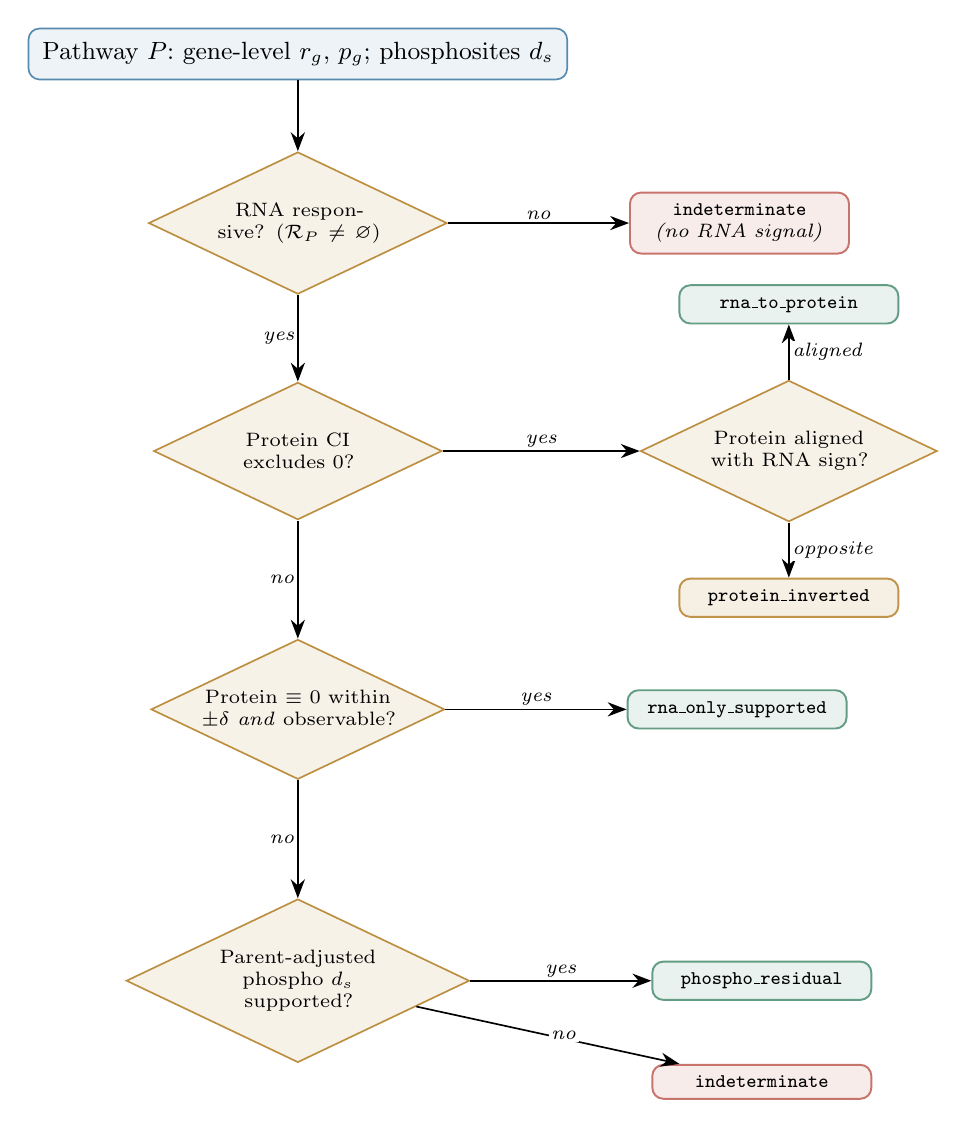
\begin{tikzpicture}
\node[start] (n0) {Pathway $P$:\ gene-level $r_g,\,p_g$; phosphosites $d_s$};
\node[decide, below=0.9cm of n0] (d1) {RNA responsive? ($\mathcal{R}_P\neq\varnothing$)};
\node[decide, below=1.1cm of d1] (d2) {Protein CI excludes $0$?};
\node[decide, below=1.5cm of d2] (d4) {Protein $\equiv 0$ within $\pm\delta$ \emph{and} observable?};
\node[decide, below=1.5cm of d4] (d5) {Parent-adjusted phospho $d_s$ supported?};

\node[termstop, right=2.3cm of d1] (tind0) {indeterminate\\ \normalfont\itshape(no RNA signal)};
\node[decide, right=2.5cm of d2] (d3) {Protein aligned with RNA sign?};
\node[termgood, above=0.7cm of d3] (tcar) {rna\_to\_protein};
\node[termstop, below=0.7cm of d3, fill=lsamber!12, draw=lsamber!80] (tinv) {protein\_inverted};
\node[termgood, right=2.3cm of d4] (trna) {rna\_only\_supported};
\node[termgood, right=2.3cm of d5] (tpho) {phospho\_residual};
\node[termstop, below=0.8cm of tpho] (tind2) {indeterminate};

\draw[flow] (n0) -- (d1);
\draw[flow] (d1) -- node[lbl,left]{yes} (d2);
\draw[flow] (d1) -- node[lbl,above]{no} (tind0);
\draw[flow] (d2) -- node[lbl,above]{yes} (d3);
\draw[flow] (d2) -- node[lbl,left]{no} (d4);
\draw[flow] (d3) -- node[lbl,right]{aligned} (tcar);
\draw[flow] (d3) -- node[lbl,right]{opposite} (tinv);
\draw[flow] (d4) -- node[lbl,above]{yes} (trna);
\draw[flow] (d4) -- node[lbl,left]{no} (d5);
\draw[flow] (d5) -- node[lbl,above]{yes} (tpho);
\draw[flow] (d5) -- node[lbl,right]{no} (tind2);
\end{tikzpicture}
\caption{\textbf{LayerScore classification decision flow.} Green = a positive evidence-backed class; amber =
inversion (evidence-backed but opposite-direction); red = abstention. Every branch that reaches
\Cind{} is a reportable outcome, not a failure. The equivalence margin $\delta$ (\S\ref{sec:delta}) governs
the \Crna{} gate.}
\label{fig:decision}
\end{figure}

% ======================================================================
\section{Statistical hazards and mitigations}
These are the failure modes that would make LayerScore produce clean but wrong answers. Each is
preregistered with its mitigation.

\subsection{Regression dilution in $\gamma_P$ (the specificity-test killer)}\label{sec:dilution}
Because $r_g$ is an estimated effect with error, the through-origin slope in Eq.~\eqref{eq:gamma} is
attenuated toward zero by approximately
\[
\frac{\sum_g w_g \rho_g^2}{\sum_g w_g \rho_g^2 + \sum_g w_g \sigma_{r,g}^2},
\]
where $\rho_g$ is the true RNA effect and $\sigma_{r,g}^2=\mathrm{Var}(r_g)$. The attenuation grows with
RNA-effect \emph{estimation error}. In the kidney-vs-muscle test (H2), tissues differ in sequencing depth
and proteome coverage, hence in $\sigma_{r,g}^2$: kidney could show ``lower carriage'' than muscle purely
because its RNA effects are noisier. This produces a publishable but false specificity claim, and it is
invisible without correction. \textbf{Mitigations, in increasing rigor:}
(a) condition the matched null on RNA-effect SE, so the null slope is attenuated identically and the
\emph{p-value} stays valid; (b) restrict $\gamma_P$ to $\mathcal{R}_P$, raising the signal-to-error ratio;
(c) use Deming / orthogonal regression with $\lambda=\sigma_p^2/\sigma_r^2$ estimated per gene from the two
SEs. At minimum, (a) is mandatory before any cross-tissue comparison.

\subsection{The equivalence margin $\delta$, and the small-$n$ reality}\label{sec:delta}
\Crna{} requires a two-one-sided-test (TOST) equivalence: the RNA-oriented protein CI must lie inside
$(-\delta,+\delta)$. $\delta$ is a \emph{smallest effect size of interest} and choosing it is the whole
method: too wide and everything is ``supported absence,'' too narrow and everything abstains. $\delta$ is
predeclared from the matched-null protein-effect scale at the relevant abundance (equivalently, the assay's
resolvable effect), and a $\delta$-sensitivity curve is reported as a result, not a footnote. \textbf{Small-$n$
consequence:} with $6$ flight / $6$ control, per-protein TMT effect CIs are wide, so in the actual RR-1 and
OSD-462 data most pathways will land in \Cind{}, and \Crna{} will be sparse. This is honest and expected;
it means the novel class is demonstrated mainly at simulation and CPTAC scale, where $n$ supports
equivalence. The paper is structured so the class earns its keep where $n$ allows.

\subsection{Parent-observability conditioning of $d_s$}
The parent-adjusted quantity in Eq.~\eqref{eq:ds} is defined only where the parent protein is quantified ---
an abundance-biased subset (abundant proteins are the detectable ones). \Cpho{} is therefore conditioned on
parent-observable proteins. The fraction of phosphosites surviving that gate is reported, and the class is
explicitly scoped to that subset. The sample-level paired model is available when phospho and protein share
samples; otherwise the higher-variance group-level fallback is used and flagged.

\subsection{RR-1 permutation floor and multiplicity}
The same-animal design admits at most $\binom{12}{6}=924$ animal-level label assignments, so the exact
permutation p-value floor is ${\approx}1/924\approx1.1\times10^{-3}$. This is adequate for a \emph{small},
preregistered pathway set or a single aggregate kidney-vs-muscle statistic, but a pathway-wide scan dies
under FDR at that floor. The specificity test commits to a handful of pathways (or one global contrast)
\emph{before} looking.

\subsection{Cross-tissue batch confounding}
If the four RR-1 tissues use different TMT plex layouts or run counts, batch is confounded with tissue and
can masquerade as layer-carriage difference. The matrix audit (Gate~2) verifies comparable designs and
confirms the same animal IDs span all four tissues, so the animal-level shared-label permutation is valid.
The observability audit is run \emph{per tissue}, separating true specificity from coverage differences.

\subsection{Conflict handling}
When $\theta_P$ (sign-oriented) and $\gamma_P$ (magnitude-weighted) disagree --- e.g., many weak-RNA genes
weakly follow while a few strong-RNA genes invert --- the pathway is routed to \Cind{} rather than forced
into a class. Disagreement between the two estimands is itself diagnostic and is logged.

% ======================================================================
\section{Novelty positioning}\label{sec:novelty}
The one-page differentiation that the method's identity depends on. If this table cannot be defended, the
method has no distinct identity and the project should stop.

\begin{center}\small
\begin{tabularx}{\textwidth}{@{}p{2.4cm} L p{3.5cm}@{}}
\toprule
\textbf{Tool} & \textbf{What it returns} & \textbf{What it does \emph{not} do} \\
\midrule
MOGSA & Unsigned per-omic \emph{contribution} to a combined single-sample gene-set score. & No directional inversion class; no null-calibrated per-pathway label; no equivalence/abstention; no parent-adjusted phospho. \\
ActivePathways & Directional \emph{merging} of per-layer p-values (evidence fusion). & Pools layers rather than localizing them; opposite of layer separation. \\
MOFA+ & Unsupervised latent factors with per-view variance explained. & Factor-level, not pathway classification; no directional carriage/inversion estimand. \\
\midrule
\textbf{LayerScore} & \textbf{A per-pathway \emph{decision}} in $\{$\Ccar{}, \Cinv{}, \Crna{}, \Cpho{}, \Cind{}$\}$ with matched-null calibration and explicit abstention. & --- \\
\bottomrule
\end{tabularx}
\end{center}
\noindent The phenomenon itself (RNA--protein buffering, attenuation, inversion) is well established in the
CPTAC literature; LayerScore's contribution is not the phenomenon but a \emph{calibrated measurement and
decision procedure} for it, with supported-absence as the differentiator.

% ======================================================================
\section{Validation hierarchy and hypotheses}

\subsection{Order of evidence}
The paper stands in this order; OSD-462 is last and is \emph{not} load-bearing.
\begin{enumerate}
\item Formal estimand and classification rules (this document).
\item Simulation with known truth --- the primary validation.
\item Controlled real benchmark with \emph{a-priori-expected} dominant layer (positive controls).
\item RR-1 kidney-vs-muscle specificity test (same-animal).
\item OSD-462 capability demonstration (recovers a known signal, abstains on a shaky one).
\end{enumerate}

\subsection{Preregistered hypotheses}
\begin{description}
\item[H1 (method).] On synthetic pathways of known class --- RNA-only, concordant, inverted, phospho-only,
protein-abundance-driven pseudo-phospho, and null --- LayerScore recovers the true class and controls false
positives, including calibrated inversion p-values and correct abstention under low coverage.
\item[H2 (comparative discovery).] Kidney RNA$\rightarrow$protein carriage differs from the consensus
response across three skeletal muscles from the same RR-1 animals, under animal-level permutation and after
controlling RNA-effect precision. \emph{A null (kidney $\approx$ muscle) is reportable.}
\item[H3 (case study).] In OSD-462, distal-transport regulation (NCC/WNK/SPAK) is classified \Cpho{} after
parent adjustment, while the broader DCT2/CNT extension is \Cind{}/scoring-sensitive.
\end{description}

% ======================================================================
\section{Data manifest}
Processed matrices only (normalized RNA counts, processed TMT tables, metadata); raw FASTQ/mass-spec are not
downloaded first.

\begin{center}\small
\begin{tabularx}{\textwidth}{@{}p{1.7cm} p{2.5cm} p{2.4cm} p{2.4cm} L@{}}
\toprule
\textbf{Accession} & \textbf{Tissue} & \textbf{Design} & \textbf{Layers} & \textbf{Role} \\
\midrule
OSD-102 & Kidney (RR-1) & 6 FLT / 6 GC & RNA, protein (TMT) & Same-animal kidney arm of H2 \\
OSD-101 & Gastrocnemius (RR-1) & same mice & RNA, protein & Muscle replicate \\
OSD-103 & Quadriceps (RR-1) & same mice & RNA, protein & Muscle replicate \\
OSD-105 & Tibialis ant.\ (RR-1) & same mice & RNA, protein & Muscle replicate \\
OSD-462 & Kidney (RR-10) & FLT / GC & RNA, protein, \textbf{phospho} & Independent phospho case (H3) \\
OSD-137 & Liver (RR-3) & within-study & RNA, protein (TMT) & Optional extension (analyze within-study) \\
CPTAC & Tumor (e.g.\ ccRCC/breast) & large $n$ & RNA, protein, phospho & Scale/robustness stress test \\
LINCS L1000/P100 & Cell perturbations & matched conditions & RNA, 96 phosphopeptides & Positive-control only (no global proteome) \\
\bottomrule
\end{tabularx}
\end{center}
\noindent \textbf{Status of OSD-102 (H2 gate).} NASA lists a processed kidney TMT archive
(\code{GLDS-102\_proteomics\_TMT\_KDNL}), TMT 10-plex over two runs, flight animals M23--M28, controls
M33--M38, with pooled reference channels (Orbitrap Fusion / Byonic). Metadata Gate~0 therefore \emph{passes}
more strongly than earlier memos assumed. What remains unverified is \emph{matrix quality} (reporter-ion
level, usable protein coverage across both runs, parseability, bridge-normalization stability, and
structural match to OSD-101/103/105). Downloading and parsing that archive is the first empirical task:
H2 has passed metadata Gate~0 but not matrix-quality Gate~1.

% ======================================================================
\section{Gated execution plan}
Each gate has a go/no-go criterion; failing a gate stops the corresponding branch, not the project
(Figure~\ref{fig:gates}). Phase~0 freezes the current v12 manuscript, outputs, environment, and tests as the
fallback paper before any refactoring.

\begin{description}
\item[Gate 1 --- Estimand memo.] Formalize carriage, inversion, and residual phosphoregulation; declare
$\delta$, equivalence criteria, coverage requirements, abstention rules, matched-null covariates, and the
handling of correlated phosphosites; state the MOGSA/ActivePathways/MOFA+ delta in one page.
\emph{No-go:} if the delta cannot be stated in a page, stop --- the method lacks an identity.
\item[Gate 2 --- Matrix audit.] Download and inspect the four RR-1 processed proteomic archives (plus
OSD-462). Tabulate samples recovered, TMT runs/channels, protein counts, missingness, shared proteins
across tissues, RNA/protein animal matching, and bridge-channel behavior. \emph{No-go:} if the four RR-1
tissues cannot be aligned by animal and platform, drop H2 (keep the method + OSD-462).
\item[Gate 3 --- Simulation (primary validation).] Generate known RNA-only, concordant, partial, inverted,
phospho-only, abundance-driven pseudo-phospho, and null pathways under realistic missingness and abundance
bias. Evaluate false-positive rate, calibration (especially of the inversion test), power, class accuracy,
whether parent adjustment separates protein drift from true phosphosite effects, whether equivalence
testing prevents small-$n$ mislabeling as \Crna{}, and the abstention rate (a result, not a nuisance).
Benchmark against RNA--protein correlation, per-layer GSEA, MOGSA, and directional ActivePathways.
\emph{No-go:} if truth is not recovered or the null is inflated, fix before any real data.
\item[Gate 4 --- Controlled real benchmark.] A perturbation dataset where the dominant layer is
\emph{expected a priori} (kinase inhibitor $\rightarrow$ \Cpho{} on substrate pathways; nuclear-receptor
agonist $\rightarrow$ \Ccar{}). This is an \emph{expectation} benchmark, not ground truth --- reserve
``known truth'' for Gate~3. CPTAC is a scale test, not causal proof.
\item[Gate 5 --- RR-1 specificity.] Animal-level label permutation shared across all tissues;
animal-cluster bootstrap intervals; TMT-run adjustment within tissue; kidney vs.\ average-muscle as the
primary contrast; individual muscles as secondary heterogeneity. Preregister the small pathway set.
\emph{Null is reportable.}
\item[Gate 6 --- OSD-462 demonstration.] Show the method flags weak RNA$\rightarrow$protein carriage, strong
regulatory-site effects, and parent-adjusted phosphoregulation for NCC/WNK/SPAK, while returning
\Cind{} for the broader DCT2/CNT extension --- a direct demonstration of the abstention principle.
Recovering an independently established signal (the NCC dephosphorylation reported by prior work) is a
\emph{feature} of a capability demo: external ground truth.
\end{description}

% ---------------- gate pipeline figure ----------------
\begin{figure}[t]
\centering
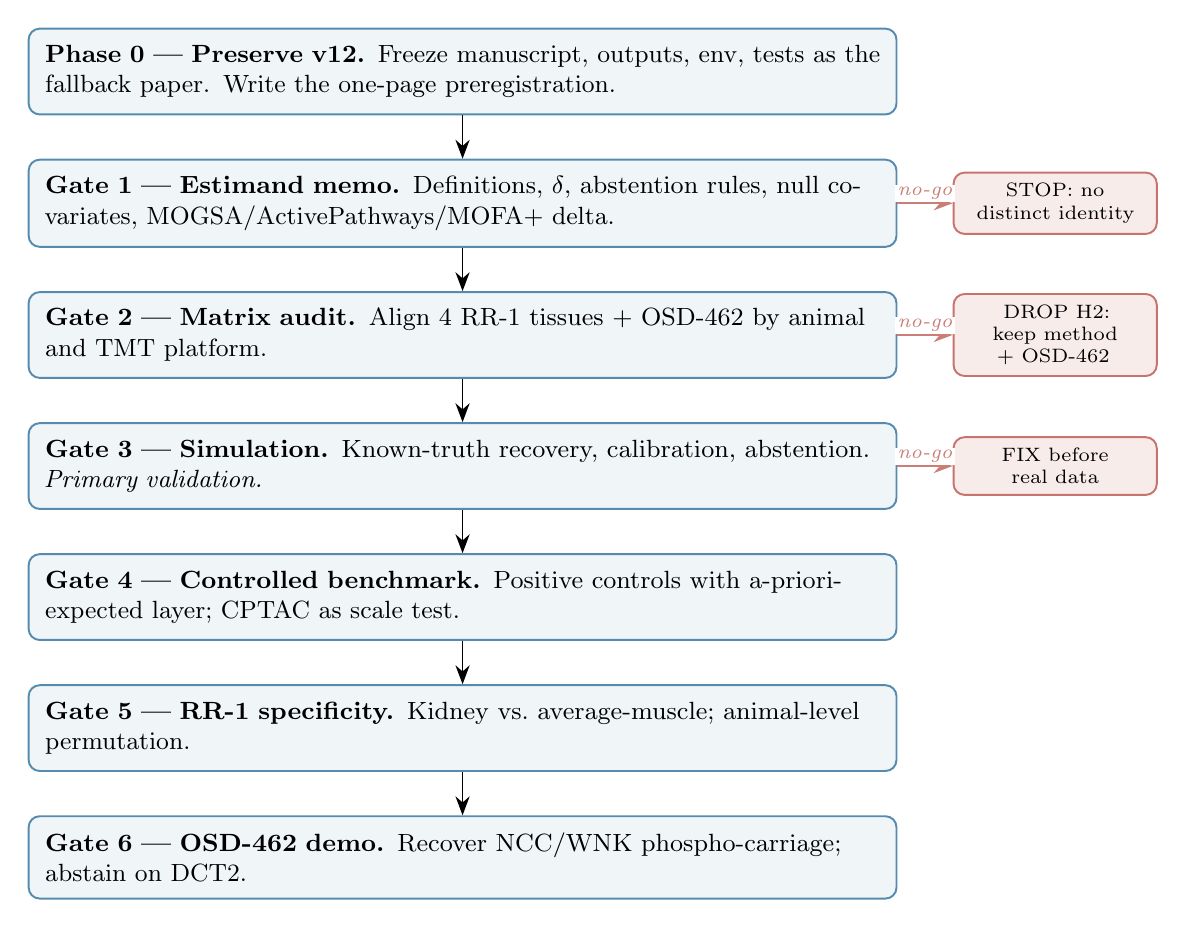
\begin{tikzpicture}
\node[gate] (g0) {\textbf{Phase 0 --- Preserve v12.} Freeze manuscript, outputs, env, tests as the fallback paper. Write the one-page preregistration.};
\node[gate, below=0.55cm of g0] (g1) {\textbf{Gate 1 --- Estimand memo.} Definitions, $\delta$, abstention rules, null covariates, MOGSA/ActivePathways/MOFA+ delta.};
\node[gate, below=0.55cm of g1] (g2) {\textbf{Gate 2 --- Matrix audit.} Align 4 RR-1 tissues + OSD-462 by animal and TMT platform.};
\node[gate, below=0.55cm of g2] (g3) {\textbf{Gate 3 --- Simulation.} Known-truth recovery, calibration, abstention. \emph{Primary validation.}};
\node[gate, below=0.55cm of g3] (g4) {\textbf{Gate 4 --- Controlled benchmark.} Positive controls with a-priori-expected layer; CPTAC as scale test.};
\node[gate, below=0.55cm of g4] (g5) {\textbf{Gate 5 --- RR-1 specificity.} Kidney vs.\ average-muscle; animal-level permutation.};
\node[gate, below=0.55cm of g5] (g6) {\textbf{Gate 6 --- OSD-462 demo.} Recover NCC/WNK phospho-carriage; abstain on DCT2.};

\node[stopnode, right=0.7cm of g1] (s1) {STOP: no distinct identity};
\node[stopnode, right=0.7cm of g2] (s2) {DROP H2: keep method + OSD-462};
\node[stopnode, right=0.7cm of g3] (s3) {FIX before real data};

\foreach \a/\b in {g0/g1,g1/g2,g2/g3,g3/g4,g4/g5,g5/g6} \draw[flow] (\a) -- (\b);
\draw[flow, lsred!70] (g1.east) -- node[lbl,above]{no-go} (s1.west);
\draw[flow, lsred!70] (g2.east) -- node[lbl,above]{no-go} (s2.west);
\draw[flow, lsred!70] (g3.east) -- node[lbl,above]{no-go} (s3.west);
\end{tikzpicture}
\caption{\textbf{Gated execution plan.} Vertical spine = the go path. Red branches = preregistered no-go
outcomes; each stops one branch, not the whole project. Gate~3 (simulation) is the primary validation and
the hard stop before any biological claim.}
\label{fig:gates}
\end{figure}

% ======================================================================
\section{Consolidated risks and limitations}
\begin{itemize}
\item \textbf{Novelty is narrow and partly pre-built.} The core scoring already exists in the repository;
all novelty must come from the formal estimand, supported-absence, the simulation, and the specificity
test. The phenomenon (buffering/inversion) is not new.
\item \textbf{$\gamma_P$ dilution} can fake H2 specificity unless the null is matched on RNA-effect precision.
\item \textbf{Small $n$} makes \Crna{} sparse in spaceflight data; the class is carried by simulation/CPTAC.
\item \textbf{Phospho is parent-gene / parent-observable resolution}, not site-localized biochemistry.
\item \textbf{OSD-462 overlaps prior published analysis}; this is acceptable \emph{only} because Gate~6 is a
capability demo, not a discovery claim.
\item \textbf{``Carriage,'' not ``propagation.''} Simultaneous RNA/protein cannot establish flow; language
stays associational throughout.
\end{itemize}

% ======================================================================
\section{Repository reuse map}
Most of the mathematical core is refactoring, not invention:
\begin{center}\small
\begin{tabularx}{\textwidth}{@{}p{5.3cm} L@{}}
\toprule
\textbf{Existing module} & \textbf{Role in LayerScore} \\
\midrule
\code{src/v11/rna\_protein\_propagation.py} & Gene classes, pathway summaries, slopes, sign agreement, matched nulls. \\
\code{src/v11/observability\_audit.py} & Abundance/missingness-aware inference; per-tissue observability. \\
\code{src/v11/matched\_null.py} & Shared null engine (currently abundance $\times$ peptide; add RNA-variance dimension). \\
\code{src/v11/h2\_occupancy\_normalized\_phospho.py} & Sample-level parent-adjusted phospho contrast (Eq.~\eqref{eq:ds}), already implemented. \\
\bottomrule
\end{tabularx}
\end{center}
\noindent Target package layout: \code{layerscore/} with \code{data.py}, \code{effects.py},
\code{scoring.py}, \code{nulls.py}, \code{phospho.py}, \code{compare.py}, \code{celltypes.py},
\code{plotting.py}, and \code{adapters/\{osdr,cptac\}.py}. The dashboard is the final 5\%, not a core aim.

% ======================================================================
\section*{Appendix: notation}
\addcontentsline{toc}{section}{Appendix: notation}
\begin{center}\small
\begin{tabularx}{\textwidth}{@{}p{2.6cm} L@{}}
\toprule
Symbol & Meaning \\
\midrule
$r_g,\,p_g$ & RNA and protein flight-contrast effects for gene $g$. \\
$\mathrm{SE}(\cdot)$ & Standard error of an effect estimate. \\
$w_g$ & Gene weight; default inverse variance $1/\mathrm{SE}(p_g)^2$. \\
$\mathcal{C}_P,\ \mathcal{R}_P$ & Co-observed genes; RNA-responsive genes of pathway $P$. \\
$\theta_P$ & Sign-oriented carriage statistic, Eq.~\eqref{eq:theta}. \\
$\gamma_P$ & Through-origin propagation slope, Eq.~\eqref{eq:gamma}. \\
$d_s$ & Parent-adjusted phosphosite effect, Eq.~\eqref{eq:ds}. \\
$\delta$ & Equivalence margin / smallest effect size of interest for \Crna{}. \\
$\sigma_{r,g}^2$ & Variance of the RNA-effect estimate (drives $\gamma_P$ dilution). \\
\bottomrule
\end{tabularx}
\end{center}

\vfill
\noindent\footnotesize\textit{Companion documents in-repo:}
\code{docs/v11\_dct2\_score\_hardening\_2026-07-10.md} (DCT2 scoring sensitivity),
\code{docs/v11\_layer\_specificity\_execution\_summary\_2026-06-07.md} (shipped propagation/observability
modules), \code{docs/v11\_gate0\_negative\_control\_search\_2026-06-07.md} (OSD-105 muscle gate), and
\code{latex\_paper/manuscript\_v12.tex} (the biology paper this method companions).

\end{document}
